\documentclass[11pt,a4paper]{article}
\usepackage[utf8]{inputenc}
\usepackage{listings}
\usepackage{hyperref}
\usepackage{graphicx}
\usepackage{tikz}

\title{Mikrokontrollerlab i Linux}
\author{TTK4235 Tilpassede Datasystemer}
\date{}

\renewcommand{\figurename}{Figur}
\renewcommand{\lstlistingname}{Kodesnutt}
\lstset{language=C, frame=single}

\begin{document}
\maketitle
\section{Bakgrunn}
\subsection{Læringsutbytte}
Denne laben er delt i tre deler, som hver skal gi en introduksjon til innvevde datasystemer, som mikrokontrollere. Del 1 vil introdusere dere til mikrokontroller IO og kommunikasjon mellom datamaskin og mikrokontroller via USART\footnote{Universal Synchronous/Asynchronous Receiver/Transmitter}. Del 2 vil ta for seg lesing av analoge signaler via en Analog/Digital-omformer (ADC). Del 3 vil bruke joysticken på kortet til å kontrollere en servomotor via PWM.

\subsection{Datablad}
For å få en mikrokontroller til å gjøre noe interessant setter man verdier i interne registre (via \textit{software}), som igjen dikterer hvordan \textit{hardware} vil oppføre seg. For å finne hvilke registre man skal sette, tar man en titt i mikrokontrollerens datablad; der står som regel alt man trenger å vite. Haken er selvsagt at datablad er svære beist som lett kan vokse seg over tusen sider, og vel så det. Derfor er det viktig å kunne finne frem til det man trenger av informasjon, slik at man unngår et nervøst sammenbrudd på lab. Heldigvis har datablader gode innholdsfortegnelser, og i Atmels tilfelle også en nyttig \textbf{registeroversikt} på slutten av hvert kapittel. Bruk denne oversikten flittig!\\
\\
Datablad for mikrokontrolleren brukt i denne laben (AT90USB1287) ligger på it's learning, men kan også finnes på Atmel sine sider.

\subsection{Linux vs. Windows}
Dere kan selv velge om dere vil bruke Windows eller Linux i denne laben. Stort sett kan forskjellene oppsummeres som i figur \ref{Win::vs:Linux}: På Windows håndterer Atmel Studio alt, mens i Linux er det fritt frem.
\begin{figure}
\centering
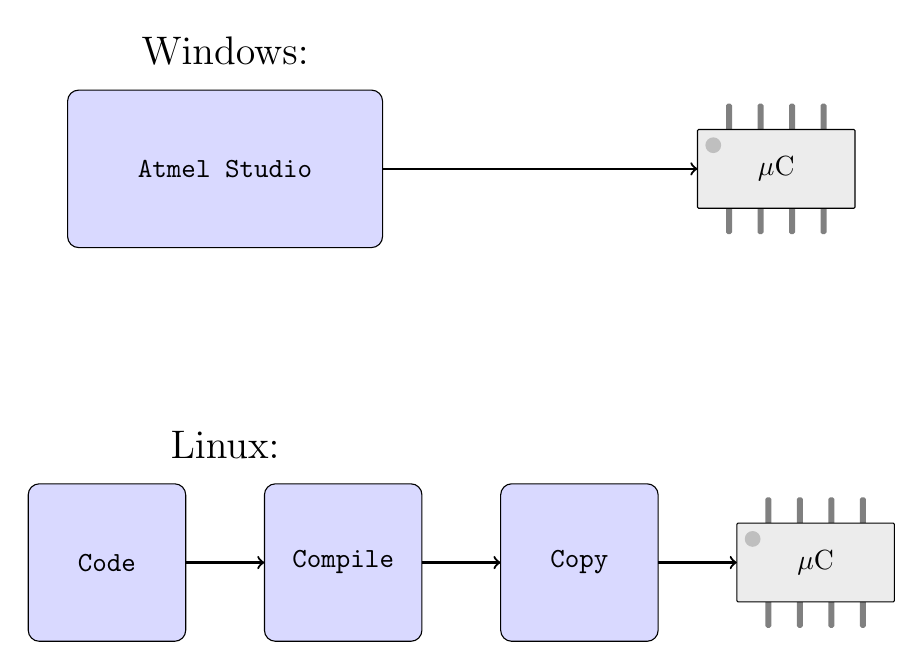
\begin{tikzpicture}[rounded corners]
\node at (2,3) {\Large Windows:};
\path[draw, fill = blue!15] (0,0.5) rectangle (4,2.5) node[midway]{\verb!Atmel Studio!};

% uC
\foreach \x in {0.4,0.8,1.2,1.6}{
\path[draw=gray, ultra thick,rounded corners=0.15] (8 + \x -0.01, 0.7) rectangle ++(0.02,1.6);
}
\path[draw, fill=gray!15,rounded corners=0.4] (8,1) rectangle ++(2,1) node[midway]{$\mu $C};
\path[fill=gray!50] (8.2,1.8) circle (0.1);

\path[draw, ->, thick] (4,1.5) -- ++(4,0);
\begin{scope}[xshift=-0.5cm]
\begin{scope}[yshift = -5cm]
\node at (2.5,3) {\Large Linux:};
\path[draw, fill = blue!15] (0,0.5) rectangle ++(2,2) node[midway]{\verb!Code!};
\path[draw, fill = blue!15] (3,0.5) rectangle ++(2,2) node[midway]{\verb!Compile!};
\path[draw, fill = blue!15] (6,0.5) rectangle ++(2,2) node[midway]{\verb!Copy!};
\begin{scope}[xshift=1cm]

% uC
\foreach \x in {0.4,0.8,1.2,1.6}{
\path[draw=gray, ultra thick,rounded corners=0.15] (8 + \x -0.01, 0.7) rectangle ++(0.02,1.6);
}
\path[draw, fill=gray!15,rounded corners=0.4] (8,1) rectangle ++(2,1) node[midway]{$\mu $C};
\path[fill=gray!50] (8.2,1.8) circle (0.1);

\end{scope}
\path[draw,->, thick] (2,1.5) -- ++(1,0);
\path[draw,->, thick] (5,1.5) -- ++(1,0);
\path[draw,->, thick] (8,1.5) -- ++(1,0);
\end{scope}
\end{scope}
\end{tikzpicture}
\caption{Windows workflow vs. Linux workflow.}
\label{Win::vs:Linux}
\end{figure}
Altså er koden og sluttresultatet likt, men om man velger Windows er man mer eller mindre låst til Atmel Studio. I Linux har man større valgmulighet - er man misfornøyd med ett av stegene involvert; står man fritt til å velge annen software som gjør samme jobb.\\
Den viktigste forskjellen er at man står fritt til å velge tekstredigeringsprogram. Hvis man er kjent med for eksempel Vim eller Emacs, er det ingen grunn til å lide under Atmel Studios klønete IDE.
\subsection{Ærlige ord basert på erfaring}
Innvevde datasystemer, eller \textit{embedded computers}, er vanskelig å komme inn i første gang. Mest sannsynlig kommer dere til å hate livet litt før dere blir kjent med databladet, og før dere kommer inn i \textit{mikrokontrollerparadigmet}. Dette er helt normalt, så fortvil ikke.\\
Laben blir ganske kul i del 3 - da faller delene på plass :)
\section{Utstyr}
\subsection{Hardware}
På starten av hver lab får dere utlevert en eske med utstyr. Denne skal inn igjen på slutten av hver lab.
\subsection{Software}
Ta vare på deres egen kode - ikke bare lagre på en lokal datamaskin og gå. Google Drive kan funke, men \href{https://git-scm.com/}{git} kombinert med \href{https://github.com/}{github} anbefales. Mange av dere er allerede kjent med git fra heisprosjektet, men om dere trenger en rask innføring kan det være lurt å ta en titt på \href{http://gitimmersion.com/}{gitimmersion.com}.
\section{Oppsett av labutstyr}
\subsection{Hardware}
\label{Setup::Hardware}
P1000-kortet som brukes i denne laben (figur \ref{p1000::card}) kan trekke strøm både fra klemmene oppe i høyre hjørne, i tillegg til USB-koblingen i høyre kant. I denne laben bruker vi USB.\\
\\
Programmering av kortet forgår via JTAG. Tidligere år har brukt en annen debugger enn det vi gjør nå, så figuren i Windows-laboppgaven er litt feil. Ta utgangspunkt i figur \ref{JTAG::conn}.
\begin{figure}[h]
\centering
\includegraphics[width=0.8\linewidth]{jtag.jpg}
\caption{Kobling av debugger til P1000-kortet.}
\label{JTAG::conn}
\end{figure}
\subsection{Software}
Dere som har valgt Linux velger fritt hvilket tekstredigeringsprogram dere ønsker å benytte. Resten av \textit{toolchainen} har vi satt opp for dere, men hvis dette er første labdag kan det hende dere må laste ned \textit{avrdude}, \textit{avr-gcc} og \textit{avr-libc}. Dette gjøres ved å kalle\\
\\
\centerline{\textbf{sudo add-apt-repository ppa:ubuntuhandbook1/apps}}
\centerline{\textbf{sudo apt-get update}}
\centerline{\textbf{sudo apt-get install -y avrdude gcc-avr avr-libc}}\\
\\
fra kommandolinjen.\\
\\
Når dette er gjort lager dere en ny mappe der dere laster ned \textit{Makefilen} fra it's learning til. Denne fungerer på samme måte som den gjorde i heisprosjektet - bare kall \textbf{make} fra kommandolinjen, så ordner \textit{gnu-make} resten.
\begin{figure}[!h]
\centering
\includegraphics[width=0.8\linewidth]{p1000.png}
\caption{P1000-kort med Atmel AT90USB1287-prosessor.}
\label{p1000::card}
\end{figure}

\section{Oppgave 1}
Koble opp kortet som beskrevet i seksjon \ref{Setup::Hardware}. Deretter kobler dere den medfølgende flatkabelen mellom \textit{PORTB} og \textit{LEDS/SW}, som indikert i figur \ref{PORTB::LEDS}. Det er viktig at den røde ledningen på flatkabelen vender i samme retning på de to tilkoblingspunktene (for eksempel til høyre hos både \textit{PORTB} og \textit{LEDS/SW}).
\begin{figure}[htb]
\centering
\includegraphics[width=0.8\linewidth]{portb_leds.png}
\caption{Koblingspunkt av flatkabel.}
\label{PORTB::LEDS}
\end{figure}
Deretter skal dere teste P1000-kortet ved å laste opp filen \textit{example.hex} som finnes på it's learning. Dette gjøres simpelthen ved å kalle \textbf{make test} fra mappen med \textit{example.hex}. Om dere får en feilmeldig, prøver dere \textbf{sudo make test}.\\
\\
Når dette er gjort skal de fire LEDene (LED0-3) til høyre på kortet blinke etter hverandre. Hvis dette ikke skjer, så huk tak i en studass.
\subsection{Knapper og LEDer}
Dere skal bruke de fire knappene til høyre på kortet til å sette av og på tilhørende lys. Lag en fil kalt \textit{main.c}. Lag også filene \textit{switch.c}, \textit{switch.h}, \textit{led.c} og \textit{led.h}. Alle \textit{c}-filene skal inkludere biblioteket $<$avr/io.h$>$.\\
\\
Følgende funksjoner skal implementeres:
\begin{itemize}
\item void init\_led()
\item void set\_led(int n, int v)
\item void init\_switch()
\item int read\_switch(int n)
\end{itemize}
De to første skal i \textit{led.c}, og de to siste skal i \textit{switch.c}. Videre skal $n$ være et tall mellom 0 og 3, som bestemmer hvilken knapp/led vi snakker om. I set\_led skal $v$ være enten 0 eller 1, som bestemmer om det skal lyse eller ikke.\\
\\
De to init-funksjonene skal sette nødvendige IO-registre før set\_led og read\_switch kalles. Alt dere trenger står i databladet under kapittel 11. Spesielt kapittel 11.1 og 11.2.1.
\subsubsection{Hint}
\begin{enumerate}
\item Både knappene og LEDene er koblet til PORTB på mikrokontrolleren. Knappene er koblet til pinne 1, 3, 5, 7. LEDene er koblet til pinne 0, 2, 4, 6.
\item LEDene er koblet i såkalt \textit{sinking mode}. Det vil si at de lyser når 0 er skrevet til pinnene i PORTB. \textit{Sourcing mode} er det motsatte.
\item Ta en titt på appendiks \ref{Bitwise::in::C} for å se hvordan vi gjør bitvis operasjoner som å sette enkelte bit i C. Særlig i kodesnutt \ref{code::names} er det inspirasjon å hente.
\end{enumerate}
\subsection{USART - Serieport}
\label{TASK::USART}
UART og USART, som står for \textbf{U}niversal (\textbf{S}ynchronous) \textbf{A}synchronous \textbf{R}eceiver \textbf{T}ransmitter, er to forkortelser som brukes litt om hverandre. Dette gjøres mest sannsynlig for å forvirre de uinnvidde.\\
Uansett årsak skal vi bruke UART til å kommunisere med datamaskinen. Koble pinne 1 på UART BRIDGE til pinne 4 på PORTD, og pinne 2 på UART BRIDGE til pinne 3 på PORTD. Se figur \ref{UART::PORTD}.
\begin{figure}[hb]
\centering
\includegraphics[width=0.8\linewidth]{uart_portd.png}
\caption{Kobling UART BRIDGE og PORTD.}
\label{UART::PORTD}
\end{figure}
Etter dette oppretter dere filene \textit{usart.c} og \textit{usart.h}. To funksjoner skal implementeres:
\begin{itemize}
\item int init\_usart(int baudrate);
\item int usart\_putchar(char c);
\end{itemize}
Baudrate betyr hvor mange bit vi sender hvert sekund. Init-funksjonen skal bare sette opp nødvendige register. Funksjonen \textit{usart\_putchar} skal først sjekke om det er klart for å sende, for så å dytte bokstaven $c$ over seriekabelen.\\
\\
Bruk følgende oppsett:
\begin{itemize}
\item Baudrate 19200.
\item Asynkron overføring.
\item Ingen paritetsbit.
\item Symbolstørrelse på 8 bit.
\end{itemize}
Alt dere trenger står i kapittel 19 i databladet, men hvis dere vil ha noe som kanskje er mer lettfattelig, så ta en titt på \href{http://extremeelectronics.co.in/avr-tutorials/using-the-usart-of-avr-microcontrollers/}{extremeelectronics.co.in}.\\
\\
Når dere er klare for å teste kobler dere P1000-kortet til datamaskinens øverste DSUB9-port. Etterpå kan dere kalle \textbf{sudo stty -F /dev/ttyS0 19200}, etterfulgt av \textbf{cat /dev/ttyS0}. Kommandoen \textbf{cat} vil bare ta hva enn som kommer inn gjennom DSUB9-porten og skrive det til skjerm.\\
\\
Om dere derimot ønsker å kunne sende ting fra datamaskinen til mikrokontrolleren kan dere kalle \textbf{minicom -b 19200 -D /dev/ttyS0}. For å gå ut fra \textbf{minicom} trykker dere \textit{Ctrl+A}, etterfulgt av \textit{Q}.\\
\\
Om dere får de bokstavene dere sender fra mikrokontrolleren inn på datamaskinen, har dere klart oppgaven.
\subsubsection{Hint}
\begin{enumerate}
\item Mikrokontrolleren kjører på 16 MHz, legg til \textbf{\#define F\_CPU 16000000UL} i toppen av \textit{uart.c}.
\item Det er lurt å sende '\textbackslash r' etterfulgt av '\textbackslash n' for å avslutte linjer sendt fra mikrokontrolleren.
\item Innholdet i registeret UBRR1 skal være $51$. Hvorfor, og vil baudraten da bli nøyaktig 19200 bits/s?
\item Feil kan oppstå både i software \textit{og} hardware. Har dere koblet riktig pinne fra UART-BRIDGE til riktig pinne på PORTD?
\end{enumerate}
\subsubsection{Frivillig oppgave}
Det går helt fin an å bruke \textit{usart\_putchar} til å sende over én og én bokstav, men det hadde vært praktisk å kunne bruke funksjonen \textit{printf} direkte. Vi kan få til dette ved å omdirigere strømmen \textit{stdout} til \textit{usart\_putchar}. Dette gjøres slik:
\begin{enumerate}
\item Legg til \textbf{static FILE usart\_stdout = FDEV\_SETUP\_STREAM( usart\_putchar, NULL, \_FDEV\_SETUP\_WRITE);} i \textit{usart.c}.
\item Legg til \textbf{stdout = \&usart\_stdout;} i slutten av \textit{init\_usart}.
\item Inkludér biblioteket $<$\textit{stdio.h}$>$ i main.
\end{enumerate}
Når dette er gjort kan dere bruke printf som dere normalt ville gjort i C-kode til vanlig. Prøv med \textit{printf("Your lucky number: \%d\textbackslash r\textbackslash n", 21)}.

\section{Oppgave 2}
Koble opp mikrokontrollerkortet med seriekabel. Kjør et program som sender bokstaver til datamaskinen og se at det fungerer, på samme måte som i avsnitt \ref{TASK::USART}. Koble deretter pinne 1 fra JOY-CONN til pinne 2 på PORTF, og pinne 2 fra JOY-CONN til pinne 1 på PORTF. Se figur \ref{JOY::PORTF}. Dette vil koble den analoge spakens X- og Y-akse til henholdsvis kanal 0 og 1 på den analoge-til-digitale omformeren i mikrokontrolleren.
\begin{figure}
\centering
\includegraphics[width=0.8\linewidth]{joystick_portf.png}
\caption{Kobling mellom analog spake og PORTF.}
\label{JOY::PORTF}
\end{figure}
\subsection{Analog/Digital-omformer}
Opprett filene \textit{adc.c} og \textit{adc.h}. Følgende to funksjoner skal implementers:
\begin{itemize}
\item void init\_adc()
\item int adc\_read(char axis)
\end{itemize}
Som før skal init-funksjonen sette opp nødvendige registre. Funksjonen \textit{adc\_read} skal ta inn \textit{axis} som bestemmer om vi skal lese av X-aksen eller Y-aksen til den analoge spaken; denne verdien skal returneres.\\
\\
I main skal dere legge til kode som periodisk leser X-posisjonen og Y-posisjonen til den analoge spaken og skriver dette ut til skjermen over USART. Sett gjerne origo til spakens nøytrale posisjon, slik at dere kan bruke $-100$ for helt til venstre/helt nede, og $+100$ for helt til høyre/helt oppe.\\
\\
All nødvendig informasjon står i kapittel 26 i databladet.
\subsubsection{Hint}
\begin{enumerate}
\item Sett referansespenningen til ADCen til AREF.
\item Bruk \textit{single conversion mode}, istedenfor \textit{freerunning mode}.
\item ADCen gir bare pålitelig 10-bits presisjon dersom den kjøres under 50 kHz - 200 kHz. Mikrokontrollerens klokke er 16 MHz. Bruk \textit{prescalers} for å ordne dette.
\item Les ADCL før dere leser ADCH når dere innhenter konvertert verdi.
\item Sett riktig bit i ADMUX hver gang dere starter en analog-til-digital omforming. Altså gjør dette i \textit{adc\_read}.
\item ADSC forblir høy helt fra en omforming startes, til den er ferdig. Dette kan brukes for å vente på resultat.
\end{enumerate}
\subsubsection{Frivillig oppgave}
Om man kontrollerer en treng enhet fra en mikrokontroller er det dumt å vente på svar via \textit{polling}. Derfor har man muligheten til å benytte \textit{interrupts}, altså at den trege enheten forteller mikrokontrolleren når den er ferdig med operasjonen den utfører.\\
\\
En ADC-konvertering tar på denne plattformen 13 ADC-klokkesykler, så \textit{interrupts} er helt overkill i dette tilfellet. Om man bruker avbruddsrutiner feil, kan faktisk mikrokontrolleren bli tregere enn om man simpelthen hadde \textit{pollet}, på grunn av unødvendig mange \textit{push}/\textit{pop}-operasjoner på tilstandsstakken.\\
\\
Uansett skal vi her svitsje fra \textit{polling} til \textit{interrupts}, bare for læringsutbyttets sin skyld. Gjør det følgende i \textit{adc.c}:
\begin{enumerate}
\item Inkludér biblioteket $<$\textit{avr/interrupt.h}$>$
\item Opprett tre global \textit{int}er, kalt \textit{global\_x}, \textit{global\_y} og \textit{x\_or\_y}.
\item Implementer funksjonen \textit{ADC\_vect()}. NB: Denne spesielle funksjonen har ingen returtype, ikke engang \textit{void}!
\item Gjør om \textit{int adc\_read} til \textit{void adc\_read}.
\item Legg til funksjonskallet \textit{sei()} i \textit{init\_adc()}. Denne funksjonen tillater \textit{globale interrupts} og er ferdig definert i \textit{avr/interrupt}.
\end{enumerate}
Dere vil nå kalle \textit{adc\_read} hver gang dere vil starte en omsetting, men dere vil ikke vente på at den blir ferdig. Hver gang dere kaller \textit{adc\_read} setter dere den globale variabelen \textit{x\_or\_y} slik at avbruddsfunksjonen vet hva den skal oppdatere når ADCen er ferdig.\\
\\
I avbruddsrutinen (\textit{ADC\_vect}) skal dere først kalle \textit{cli()}, denne funksjonen er motsatt av \textit{sei()} og sørger for at dere ikke får en ny interrupt mens dere behandler denne. Last deretter verdien som ligger ferdig i ADCL og ADCH inn i enten \textit{global\_x} eller \textit{global\_y}, avhengig av verdien til \textit{x\_or\_y}. På slutten av avbruddsrutinen må dere huske på å skru på globale avbrudd med \textit{sei()}, slik at \textit{adc\_read} fortsatt vil fungere etterpå.\\
\\
Når dere er ferdige med alt dette kan dere simpelthen sende \textit{global\_x} og \textit{global\_y} over seriekabelen. Som sagt så er avbruddsrutiner rett og slett tull og tøys i dette tilfellet, men dersom man for eksempel styrer \textit{flere, trege eksterne ADCer} fra én og samme mikrokontroller - da kan \textit{interrupts} være en god idé.

\section{Oppgave 3}
I denne oppgaven skal dere få en servomotor til å følge posisjonen til den analoge spaken på mikrokontrollerkortet. For å oppnå dette, skal vi bruke mikrokontrollerens innebygde PWM-modul. Mange servomotorer, inkludert denne, forventer en svitsjeperiode på $20\,\mathrm{ms}$ - som betyr at vi trenger en frekvens på $50\,\mathrm{Hz}$. Pulsbredden til signalet vil avgjøre hvilken vinkel motoren får, lav \textit{duty cycle} gir liten vinkel, høy \textit{duty cycle} gir stor vinkel. Se figur \ref{Servo::PWM}.\\
\\
Pass på at pulsbredden til styresignalet deres ikke går utenfor området $0.9 - 2.1\,\mathrm{ms}$, hvis ikke kan servomotoren ødelegges.
\begin{figure}[h]
\centering
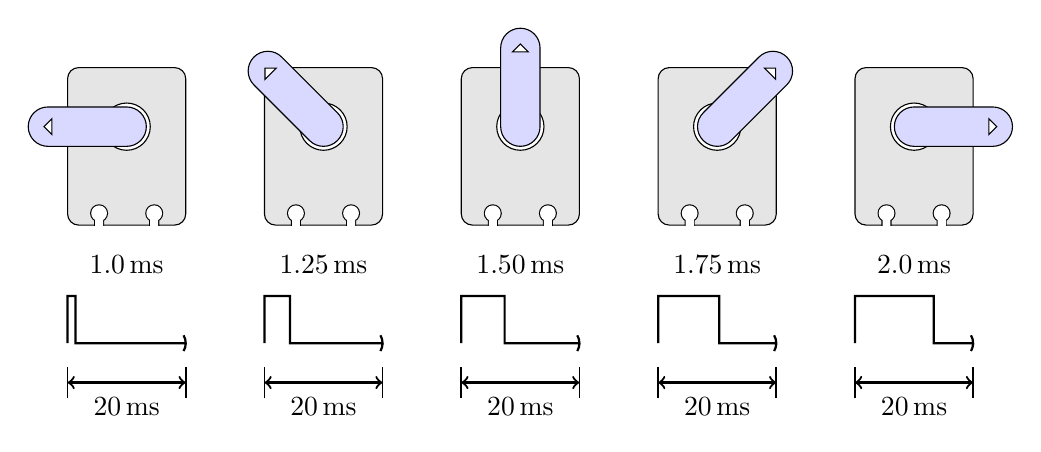
\begin{tikzpicture}
%% Colors
\colorlet{secCol}{blue!15};
%% Servo arm
\tikzset{pics/arm/.style args={#1}{
code = {
\begin{scope}[scale=0.5,xshift=-1cm,yshift=1.5cm,rotate around={#1:(2.5,1)}]
\path[draw, fill=white] (2.5,1) circle (0.6);
\path[draw, fill = secCol] (0.5,0.5) arc (270:90:0.5) -- ++(2,0)  arc (90:-90:0.5) -- cycle;
\path[draw, fill=white] (0.5,1) ++ (-0.1,0) -- ++ (0.2,0.2) -- ++(0,-0.4) -- cycle;
\end{scope}
}
}
}
%% Motor box
\tikzset{box/.pic = {
\path[draw,thin,rounded corners,fill=gray!20] (0,0) rectangle ++ (1.5,2);
\begin{scope}
\path[clip] (0,0) rectangle ++(1.5,2);
\path[draw,thick,postaction={fill=white}] (0.35,0.1) rectangle ++(0.1,-0.2) ++(-0.05,0.25) circle (0.1);
\path[draw,thick,postaction={fill=white}] (1.05,0.1) rectangle ++(0.1,-0.2) ++(-0.05,0.25) circle (0.1);
\end{scope}
\path[fill=white] (1.05,0.1) rectangle ++(0.1,-0.2);
\path[fill=white] (0.35,0.1) rectangle ++(0.1,-0.2);
}
}

\foreach \x/\rot/\duty/\val in {0/0/0.1/1.0,
2.5/-45/0.325/1.25,
5/-90/0.55/1.50,
7.5/-135/0.775/1.75,
10/-180/1/2.0}{
% Servo motors
\path (\x,0) pic {box};
\path (\x,0) pic {arm=\rot};

% Duty cycles
\path[draw,thick] (\x,-1.5) -- ++(0,0.6) -- ++(\duty,0) -- ++ (0,-0.6) -- (\x + 1.5,-1.5)
arc (0:30:0.2) arc (30:-30:0.2);
\node at (\x + 0.75,-0.5) {$\val\,\mathrm{ms}$};

% Switch periodes
\path[draw,thick,<->] (\x,-2) -- ++(1.5,0);
\path[draw,semithick] (\x,-2.2) -- ++(0,0.4) ++ (1.5,0) -- ++(0,-0.4);
\node at (\x + 0.75,-2.3) {$20\,\mathrm{ms}$};
}


\end{tikzpicture}
\caption{Pulsbreddesignal inn på servomotor med tilhørende vinkel.}
\label{Servo::PWM}
\end{figure}
\subsection{Pulsbreddemodulasjon}
Først oppretter dere filene \textit{pwm.c} og \textit{pwm.h}. Følgende funksjoner skal implementeres:
\begin{itemize}
\item void init\_pwm()
\item void pwm\_set\_duty(double ms)
\end{itemize}
Som før skal init-funksjonen sette alle nødvendige registre. Funksjonen \textit{pwm\_set\_duty} skal ta inn en \textit{double} i området $1.0$ til $2.0\,\mathrm{ms}$, slik at dere har en feilmargin på $0.1\,\mathrm{ms}$ i begge ender, før servoen ryker.\\
\\
Dere skal bruke \textbf{Timer1} på mikrokontrolleren. Utgangen på denne er koblet til \textbf{OC1A}; ta en titt i databladet for å finne ut hvilken IO-pinne dette svarer til. Denne pinnen må settes i \textit{output}-modus.\\
\\
Tanken er at vi skal kunne bruke PWM-modulen som illustrert i figur \ref{PWM::14}. Vi skal kunne sette en verdi i registeret \textbf{ICR1}, som den interne telleren skal telle opp til. Når telleren når denne verdien skal den starte på nytt, samtidig som den setter et høyt utgangssignal. Vi skal kunne bestemme pulsbredden ved å skrive en verdi til registeret \textbf{OCR1A}. Når telleren når denne verdien, skal utgangssignalet gå lavt.\\
\\
Ta en titt på kapittel 15 i databladet for å finne ut hva du må sette. Spesielt er tabell 15.2 og 15.4 til stor hjelp.
\begin{figure}[h]
\centering
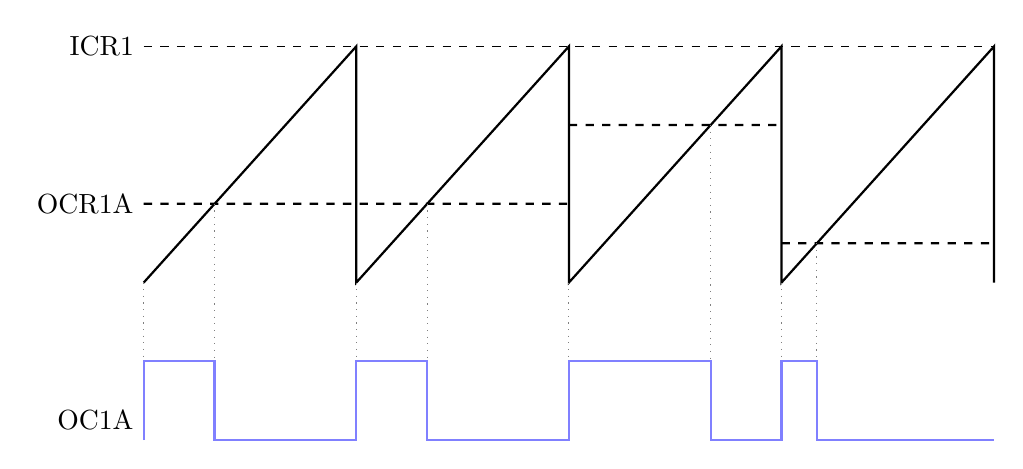
\begin{tikzpicture}[xscale=0.9]
% Internal counter
\path[draw,thick] (0,2) --++(3,3) --++(0,-3) --++(3,3) --++(0,-3) --++(3,3) --++(0,-3) --++(3,3) --++(0,-3);
% ICR1
\path[draw,dashed] (0,5)  node[left] {ICR1} --(12,5);
% OCR1A
\path[draw,thick,dashed] (0,3) node[left] {OCR1A} -- (6,3)++ (0,1) -- (9,4) ++ (0,-1.5) -- (12,2.5);
% OC1A
\path[draw=blue!50,thick] (0,0) node[above left] {OC1A} --++ (0,1)--++(1,0)--++(0,-1)--++(2,0)--++(0,1)--++(1,0)
--++(0,-1)--++(2,0)--++(0,1)--++(2,0)--++(0,-1)--++(1,0)--++(0,1)--++(0.5,0)--++(0,-1)--++(2.5,0);
% Resets
\begin{scope}[draw=gray,dotted]
\foreach \x in {0,3,...,9}{
\draw (\x,2) --++(0,-1);
}
\draw (1,3) -- (1,1);
\draw (4,3) -- (4,1);
\draw (8,4) -- (8,1);
\draw (9.5,2.5) -- (9.5,1);
\end{scope}
\end{tikzpicture}
\caption{Ønsket pulsbreddemodulasjonsvirkemåte.}
\label{PWM::14}
\end{figure}
For å få riktig svitsjeperiode må dere bruke \textit{prescalers}, hvis ikke ville en periode blitt $4.1\,\mathrm{ms}$. Ta en titt i tabell 15.5 for å finne en egnet \textit{prescaler}.\\
\\
Når dere har satt opp alt kobler dere et oscilloskop på utgangspinnen til \textbf{OC1A} og måler perioden. Dytt også den analoge spaken ut i kantene og forsikre dere om at det er umulig å få en \textit{duty cycle} utenfor det sikre området.
\subsubsection{Hint}
\begin{enumerate}
\item Den riktige PWM-modusen er en av \textit{Fast PWM}-modiene.
\item Om dere får feil \textit{duty cycle} på utgangen, så er to vanlige feilkilder \textit{heltallsdivisjon} og \textit{overflyt} i \textit{pwm\_set\_duty}.
\item To forskjellige \textit{prescalers} fungerer godt i dette tilfellet her; dere bør velge den minste. Hvorfor?
\end{enumerate}
\subsection{Servomotorkontroll}
Dette er øyeblikket alle har ventet på! Timene med intens databladlesing vil nå være verd innsatsen. Det vil være noen grønne motorbokser tilgjengelig på Sanntidssalen. Servomotoren i denne boksen har følgende tre ledninger: \textbf{gul} (PWM), \textbf{rød} ($V_{CC}$), og \textbf{svart} (jord). Koble disse til P1000-kortet.\\
\\
Dere vil nå kunne styre servomotoren ved hjelp av den analoge spaken.
\subsubsection{Hint}
\begin{enumerate}
\item Samme signalisering kan brukes til å kontrollere en \textit{micro servo}, for eksempel den sett i figur \textcolor{red}{Insert this}. Koble denne til en mikrokontroller med bluetooth, og dere har en trådløs lysbryter.
\item Dere vil se mer enn nok av mikrokontrollerkortet igjen i TTK4155, "byggern".
\item Omega Verksted har stort sett de komponentene dere skulle trenge, og kunnskapen til å hjelpe dere, om dere ønsker å utforske innvevde datasystemer på egenhånd. Dette er en veldig god måte å lære på :)
\end{enumerate}

\newpage
\noindent
\appendix
\section{Bitoperasjoner i C}
\label{Bitwise::in::C}
C har følgende bitvise operatorer:
\begin{itemize}
\item[\&] - Bitvis \textbf{og}
\item[\textbar] - Bitvis \textbf{eller}
\item[\textasciicircum] - Bitvis \textbf{XOR} (exclusive or)
\item[\textasciitilde] - Bitvis \textbf{ikke} (not)
\item[$<<$] - Venstreskift
\item[$>>$] - Høyreskift
\end{itemize}
Et eksempel på hvordan disse operatorene virker er gitt i kodesnutt \ref{code::bitwise}. Du forstår best hvordan koden i snutt \ref{code::bitwise} fungerer hvis du skriver opp eksemplene selv og gjør de for hånd!
\begin{lstlisting}[caption=Bitvise operatorer i C.,label=code::bitwise]
// Prefix 0b means number in binary
char a = 0b10101010;
char b = 0b11110000;
char c;

c = a | b;		// c is now 0b11111010
c = a & b;		// c is now 0b10100000
c = b >> 2;		// c is now 0b00111100
c = a ^ b;		// c is now 0b01011010
c = ~b;			// c is now 0b00001111
\end{lstlisting}
Når vi programmerer mikrokontrollere setter vi ofte ett enkelt bit på eller av i et register. Dette gjøres ofte på følgende måte:
\begin{lstlisting}[caption=Setting av enkelte bit.,label=code::setting]
char c = 0b10000001;

// To set bit 3 from right side, we do:
c |= (1 << 2);		// c is now 0b10000101

// To clear it agin, we do:
c &= ~(1 << 2);		// c is now 0b10000001
\end{lstlisting}
Igjen: Du lærer hvordan koden i snutt \ref{code::setting} fungerer ved å gå gjennom den for hånd.\\
\\
På mikrokontrolleren brukt i denne laben er registrene 8 bit, og kan fint settes på måten vi gjorde i kodesnutt \ref{code::setting}. Dette er imidlertid bare tull, fordi koden blir helt uoversiktlig. For å gjøre jobben din enklere har hvert register og hvert bit i hvert register sitt eget navn. Disse navnene er definert i biblioteket \textit{avr/io}. Slik bruker vi det:
\begin{lstlisting}[caption=Bruk av registernavn.,label=code::names]
#include <avr/io.h>
...

// To set bit PB0 in DDRB
DDRB |= (1 << PB0);

// To clear bit PB0 in PORTB
PORTB &= ~(1 << PB0);
\end{lstlisting}
I kodesnutt \ref{code::names} demonstrerer vi hvordan vi setter pinne 0 i \textbf{D}ata-\textbf{D}irection-\textbf{R}egister-\textbf{B}, slik at pinne 0 blir satt i \textit{output}-modus. Deretter skrur vi av pinne 0 i PORTB, slik at pinnen er logisk lav.
\end{document}